%! Author = Omar Iskandarani
%! Date = 12/3/2025
%! Affiliation = Independent Researcher, Groningen, The Netherlands
%! License = © 2025 Omar Iskandarani. All rights reserved. This manuscript is made available for academic reading and citation only. No republication, redistribution, or derivative works are permitted without explicit written permission from the author. Contact: info@omariskandarani.com
%! ORCID = 0009-0006-1686-3961
%! DOI = 10.5281/zenodo.xxx

\newcommand{\paperdoi}{10.5281/zenodo.xxx}
\newcommand{\papertitle}{{Multi–Scale Thermodynamics of the Swirl Condensate}}\\[4pt]
{\large A Unified Hydrodynamic–Topological Framework for Swirl–String Theory}

%=========================================
% PREAMBLE, PACKAGES AND DOCUMENT CONFIGURATION
%=========================================
\documentclass[11pt]{article}
\usepackage{amsmath,amssymb,amsfonts,bm}
\usepackage{siunitx}
\usepackage[hidelinks]{hyperref}
\usepackage[a4paper,margin=1in]{geometry}
\usepackage[T1]{fontenc}
\usepackage[utf8]{inputenc}
\usepackage{tikz}

% swirl arrows (context-aware)
\newcommand{\swirlarrow}{\mkern-2mu\scriptscriptstyle\boldsymbol{\circlearrowleft}}
\newcommand{\vswirl}{\mathbf{v}_{\swirlarrow}}
\newcommand{\SwirlClock}{S_{(t)}^{\swirlarrow}}
\newcommand{\Fmaxswirl}{F^{\max}_{\mkern-1mu\scriptscriptstyle\boldsymbol{\circlearrowleft}}}
% swirl arrows Counter Clockwise
\newcommand{\swirlarrowcw}{ \mkern-2mu\scriptscriptstyle\boldsymbol{\circlearrowright}}
\newcommand{\vswirlcw}{\mathbf{v}_{\swirlarrowcw}}
\newcommand{\SwirlClockcw}{S_{(t)}^{\swirlarrowcw}}
\newcommand{\Fmaxswirlcw}{F^{\max}_{\mkern-1mu\scriptscriptstyle\boldsymbol{\circlearrowright}}}

\newcommand{\Fmax}{\Fmaxswirl} % default maximal force (left swirl)
\newcommand{\FmaxEM}{F^{\max}_{\mathrm{EM}}}
\newcommand{\FmaxG}{F_{\mathrm{G}}^{\max}}               % G-like maximal force scale

\newcommand{\omegas}{\boldsymbol{\omega}_{\swirlarrow}}  % swirl vorticity
\newcommand{\Om}{\Omega_{\swirlarrow}}                   % swirl angular frequency profile

\newcommand{\vscore}{v_{\swirlarrow}}                    % shorthand: |v_swirl| at r=r_c
\newcommand{\vnorm}{\lVert \mathbf{v}_{\swirlarrow} \rVert}               % swirl speed magnitude
\newcommand{\Ce}{\vswirl}                                % canonical swirl-speed constant

\newcommand{\rhof}{\rho_{\!f}}                           % effective fluid density
\newcommand{\rhoE}{\rho_{\!E}}                           % swirl energy density
\newcommand{\rhom}{\rho_{\!m}}                           % mass-equivalent density
\newcommand{\rc}{r_c}                                    % string core radius (swirl string radius)

\newcommand{\rhoM}{\rho_{\!m}}          % mass-equivalent density
\newcommand{\rhocore}{\rho_{\text{core}}}


\newcommand{\Lam}{\Lambda}                               % Swirl Coulomb constant
\newcommand{\alpg}{\alpha_g}                             % gravitational fine-structure analogue

\newcommand{\titlepageOpen}{
    \begin{titlepage}
    \thispagestyle{empty}
    \centering
    \Large \bfseries \papertitle \par \vspace{1cm}
    {\Large \itshape \textbf{Omar Iskandarani}\textsuperscript{\textbf{*}} \par}
    \vspace{0.5cm}
    {\today \par}
    \vspace{0.5cm}
}

\newcommand{\titlepageClose}{
    \vfill \raggedright \null
    \begin{picture}(0,0)
    \put(0,-45){  % Shift 200pt left, 40pt down
        \begin{minipage}[b]{0.7\textwidth} \footnotesize
        \renewcommand{\arraystretch}{1.0}
        \noindent\rule{\textwidth}{0.4pt} \\[0.5em]
        \textsuperscript{\textbf{*}} Independent Researcher, Groningen, The Netherlands \\
        Email: \texttt{info@omariskandarani.com} \\
        ORCID: \texttt{\href{https://orcid.org/0009-0006-1686-3961}{0009-0006-1686-3961}} \\
        DOI: \href{https://doi.org/\paperdoi}{\paperdoi}
        \end{minipage}
    }
    \end{picture}
    \end{titlepage}
}
%=========================================
% Start Document - Title Page
%=========================================
\begin{document}
    \titlepageOpen
    \begin{abstract}
        We develop a comprehensive thermodynamic formulation of Swirl–String Theory (SST),
        in which the physical vacuum is modeled as a frictionless, incompressible swirl
        condensate, and all matter arises as topologically stabilized vortex filaments
        (``swirl strings''). Building on the quantum–thermodynamic isomorphism of Abe \&
        Okuyama, we demonstrate that hydrogenic structure, particle masses, vacuum
        fluctuations, and interaction lifetimes can be reinterpreted as thermodynamic
        processes involving the swelling, compression, and mode–excitation of vortex
        cores.

        We define SST Work as the mechanical energy required to deform the vortex core
        radius against the surrounding swirl pressure, and SST Heat as the energy
        redistributed among Kelvin modes and topological phase channels. Applying this
        framework to hydrogen, we show that the Bohr radius is not a probabilistic orbital
        shell but a thermodynamic equilibrium surface where centrifugal swirl pressure
        balances vacuum tension.

        We reinterpret the Golden Layer mass hierarchy as a discrete thermodynamic
        scaling law governed by the golden ratio, emerging from log–periodic structure in
        the swirl energy density. The Unruh Echo is shown to arise from a two–stage
        thermodynamic response: a 0.1 ns vorticity burst followed by a delayed
        electromagnetic transduction pulse around 30 ns. Finally, we derive partition
        functions, heat capacities, and provide numerical evaluation for a simplified
        Golden ladder.
    \end{abstract}

    \titlepageClose
%=========================================
% Title Page End
%=========================================
%==============================================================
%  MULTI-SCALE THERMODYNAMICS OF THE SWIRL CONDENSATE — DEEL I
%==============================================================
--------------------------------------------

%==============================================================
    \section{Introduction: The Hydrodynamic Necessity}
%==============================================================

        \subsection{Ontological Divergence in Modern Physics}

            General Relativity models gravity as spacetime curvature, while Quantum Field
            Theory models matter as excitations of an operator–valued vacuum. These
            frameworks are empirically successful yet mathematically incompatible.

            Swirl–String Theory (SST) replaces both ontologies with a physical one: the
            vacuum is a real fluid with density, pressure, vorticity, and circulation. Matter
            is reinterpreted as knotted vortex filaments of this medium. Mass, time dilation,
            charge, binding energy and field structure all emerge as hydrodynamic responses.

        \subsection{The Thermodynamic Hypothesis}

            SST has precise formulations for kinematics, field analogues, knot mass spectra,
            and hydrogen structure, but lacks a unifying thermodynamic interpretation.
            Abe \& Okuyama showed that the Schrödinger equation can be reformulated as a
            thermodynamic equation of state if one assigns Shannon entropy to the quantum
            probabilities and imposes the Clausius equality. Their mapping between
            probability flows and thermodynamic heat is the missing bridge for SST.

        \subsection{Objectives of this Framework}

            Our aims:

            \begin{enumerate}
                \item Define the swirl string as a thermodynamic system embedded in a reservoir.
                \item Identify its thermodynamic variables: core radius, Kelvin modes, topology.
                \item Define SST Work as geometric deformation of $r_c$.
                \item Define SST Heat as Kelvin–mode or R/T–phase redistribution.
                \item Derive the SST equation of state from Euler--Bernoulli and circulation laws.
                \item Map Abe–Okuyama adiabatic/isothermal processes to SST swelling dynamics.
                \item Apply the framework to hydrogen, Golden Layers, Unruh Echo and partition
                functions.
            \end{enumerate}

%==============================================================
    \section{The Hydrodynamic Substrate: Axioms and Constants}
%==============================================================

        \subsection{The Primitive Triad}

            SST is based on three primitive medium parameters:

            \begin{itemize}
                \item Circulation quantum:
                \[
                    \Gamma_0 \approx 6.4 \times 10^3 \ \mathrm{m^2/s}.
                \]

                \item Core radius:
                \[
                    r_c \approx 1.41 \times 10^{-15} \ \mathrm{m}.
                \]

                \item Effective fluid density:
                \[
                    \rho_f \approx 7.0 \times 10^{-7} \ \mathrm{kg/m^3}.
                \]
            \end{itemize}

            Via circulation conservation $\Gamma = v r$, this yields the swirl speed scale
            \[
                v_{\!\circlearrowleft} = \frac{\Gamma_0}{2\pi r_c}
                \approx 1.09 \times 10^6 \ \mathrm{m/s}.
            \]

            This is the characteristic ``sound'' speed of swirl excitations.

        \subsection{The Mass Kernel as Equation of State}

            SST mass arises from the hydrodynamic energy of the vortex:

            \[
                M(T) = \Lambda_0 \, \mathcal{I}_M(K(T)) \, L_{\rm tot}(T),
            \]

            with $\Lambda_0 \propto \rho_f v_{\!\circlearrowleft}^2 r_c^3$, a topological
            invariant $\mathcal{I}_M$, and total ropelength $L_{\rm tot}$.
            Thus rest mass is interpreted as stored adiabatic work.

        \subsection{The Swirl Clock}

            Time dilation follows:
            \[
                S_t = \sqrt{1 - \frac{v^2}{c^2}}.
            \]
            Since $v \sim 1/r$, smaller radii produce larger speeds and slower clocks.
            This couples energy density directly to local temporal flow.

%==============================================================
    \section{The Quantum–Thermodynamic Isomorphism (Abe–Okuyama)}
%==============================================================

        \subsection{Particle in a Box vs. Vortex in a Core}

            Quantum energies scale as:
            \[
                E_n(L) \propto \frac{1}{L^2}.
            \]
            Vortex energies scale as:
            \[
                E(r_c) \propto \frac{1}{r_c^2}.
            \]
            Hence the mappings:
            \[
                L \leftrightarrow r_c, \qquad
                |u_n\rangle \leftrightarrow \text{Kelvin modes}.
            \]

        \subsection{Mapping of Variables}

            \begin{center}
                \begin{tabular}{lll}
                    \hline
                    Abe--Okuyama          & SST Equivalent        & Interpretation \\
                    \hline
                    Well width $L$        & Core radius $r_c$     & Confinement scale \\
                    Probabilities $p_n$   & Kelvin mode weights   & Microstates \\
                    Heat                  & $\sum E_n dp_n$       & Mode excitation \\
                    Work                  & $\sum p_n dE_n$       & Core deformation \\
                    Entropy               & Shannon entropy        & Topological complexity \\
                    \hline
                \end{tabular}
            \end{center}

        \subsection{First and Second Laws}

            Quantum variation:
            \[
                dE = \sum_n E_n dp_n + \sum_n p_n dE_n.
            \]

            Thus:
            \[
                \delta Q = \sum_n E_n dp_n, \qquad
                \delta W = \sum_n p_n dE_n.
            \]

            In SST:
            \begin{itemize}
                \item Heat = redistribution of Kelvin modes.
                \item Work = deformation of $r_c$.
            \end{itemize}

%==============================================================
    \section{Multi-Scale Thermodynamics of the Swirl Condensate}
%==============================================================

        \subsection{The Swirl String as Thermodynamic System}

            The swirl string is immersed in the swirl condensate reservoir.
            Thermodynamic variables:

            \begin{itemize}
                \item $r_c$: geometric confinement coordinate.
                \item $\{p_n\}$: Kelvin–mode populations.
                \item Topological sector $K$: conserved under adiabatic evolution.
            \end{itemize}

        \subsection{SST Work: Core Deformation}

            Euler’s radial momentum equation gives:
            \[
                \frac{dp}{dr} = \rho_f \frac{v_\theta^2}{r},
                \quad
                v_\theta = \frac{\Gamma}{2\pi r}.
            \]
            Integrating:
            \[
                p(r) = p_\infty - \frac12 \rho_f v_\theta^2.
            \]

            Thus the compressive tension at $r_c$ scales as:
            \[
                p(r_c) \propto \frac{1}{r_c^2}.
            \]

            Work associated with changing $r_c$:
            \[
                \delta W_{SST} = \left( \frac{\partial H}{\partial r_c} \right) dr_c
                \propto \frac{dr_c}{r_c^3}.
            \]

        \subsection{SST Heat: Kelvin Mode Excitation}

            At fixed geometry:
            \[
                \delta Q_{SST} = \sum_n E_n(r_c)\, dp_n.
            \]

            Heat corresponds to:
            \begin{itemize}
                \item mode activation,
                \item Kelvin–helix excitations,
                \item R/T phase reconfigurations.
            \end{itemize}

        \subsection{Adiabatic vs. Isothermal Swelling}

            Adiabatic (entropy fixed, topology protected):
            \[
                f r_c^3 = \mathrm{const}.
            \]

            Isothermal (vacuum temperature fixed):
            \[
                f r_c = \mathrm{const}.
            \]

            Hydrogen formation proceeds isothermally; rest mass originates adiabatically.

%==============================================================
% END DEEL I
%==============================================================

%==============================================================
%  MULTI-SCALE THERMODYNAMICS OF THE SWIRL CONDENSATE — DEEL II
%==============================================================

%==============================================================
    \section{Application I: Thermodynamic Origin of Hydrogen Structure}
%==============================================================

        \subsection{Two-Scale Geometry: $r_c \rightarrow a_0$}

            A swirl string representing the electron possesses two relevant geometric scales:

            \[
                r_c \approx 1.41 \times 10^{-15}\ \mathrm{m}, \qquad
                a_0 \approx 5.29 \times 10^{-11}\ \mathrm{m}.
            \]

            The SST Canon provides the scaling relation:
            \[
                a_0 = \frac{c^2}{2\,v_{\!\circlearrowleft}^2}\, r_c,
            \]
            which quantitatively reproduces the Bohr radius.
            Thus the electronic vortex undergoes a thermodynamic expansion from
            $r_c$ to $a_0$ during atom formation.

        \subsection{Hydrogen Formation as an Isothermal Expansion}

            During hydrogen binding, the electron vortex moves inward toward the protonic
            swirl–Coulomb potential. The relevant force is a compressive hydrodynamic
            pressure:

            \[
                P(r) = P_\infty - \frac12 \rho_f v_\theta^2(r),
                \quad
                v_\theta = \frac{\Gamma_0}{2\pi r}.
            \]

            As $r$ decreases, $v_\theta$ increases, lowering the internal pressure at the
            core boundary and generating a net inward force.

            Thermodynamically, this corresponds to \emph{mechanical work} performed on the
            swirl string. However, the system must remain in equilibrium with the
            reservoir's swirl fluctuations. Thus, binding proceeds through an isothermal
            process.

            The equilibrium point occurs when:

            \[
                \frac{dF}{dr} = 0,
                \quad
                F = E - T_{\rm sw} S,
            \]

            with $S$ the topological/Kelvin entropy and $T_{\rm sw}$ the swirl reservoir
            temperature. This yields precisely $r = a_0$ as the stable radius.

        \subsection{Clock Rate Difference: Cold vs. Hot States}

            The swirl clock:
            \[
                S_t(r) = \sqrt{1 - \frac{v_\theta^2(r)}{c^2}}
            \]
            implies:

            \begin{itemize}
                \item Small $r$: large swirl speed, strong time dilation.
                \item Large $r$: weaker swirl, faster internal clock.
            \end{itemize}

            Thus the hydrogen ground state (at $a_0$) is not only an energy minimum, but a
            \emph{slow-clock minimum}. Excited states have larger radii and therefore
            experience less time dilation, accelerating spontaneous decay.

        \subsection{Hydrogen as Thermodynamic Boundary Balance}

            Hydrogen is stable because:

            \[
                \frac12 \rho_f v_\theta^2(a_0)
                \quad \text{balances} \quad
                P_{\mathrm{vac}},
            \]

            and any small displacement increases free energy.
            Thus atomic structure is fundamentally a thermodynamic equilibrium of swirl
            pressure and vacuum tension.

%==============================================================
    \section{Application II: Thermodynamics of the Golden Layer}
%==============================================================

        \subsection{The Golden Ratio as Critical Thermodynamic Exponent}

            The SST mass functional includes a Golden suppression factor:
            \[
                M(K) \propto \phi^{-g(K)} n(K)^{-1/\phi},
            \]
            with $g$ the genus and $n$ the number of components.
            This resembles a Boltzmann factor:
            \[
                e^{-\Delta E / kT}
                \;\; \leftrightarrow \;\;
                \phi^{-g}.
            \]

            Thus high–genus topologies are \emph{thermodynamically suppressed} in the swirl
            condensate. Mass emerges from the competition between:

            \begin{itemize}
                \item geometric stretching energy (ropelength),
                \item vacuum displacement energy,
                \item topological entropy measured by Golden scaling.
            \end{itemize}

        \subsection{Golden Potential and Log-Periodic Structure}

            Define the Golden potential for swirl energy density $\rho_E$:
            \[
                V_\phi(\rho_E)
                = \Lambda^4 \left[
                                1 - \cos\!\left(
                                              \frac{2\pi}{\ln\phi}
                                              \ln\!\frac{\rho_E}{\rho_E^\ast}
                    \right) \right].
            \]

            Since $\rho_E \propto 1/r^2$, the core stability inherits a log–periodic
            structure:

            \[
                r_{n+1} = r_n\,\phi.
            \]

            These are the ``Golden Layers''—thermodynamic attractors of the vortex core.

        \subsection{Fractal Heat Capacity}

            A log–periodic system has a heat capacity of the form:
            \[
                C_V(T)
                = C_0 \left[
                          1 + A \cos\!\left(
                                          \frac{2\pi}{\ln\phi}
                                          \ln\!\frac{T}{T_\ast}
                                          + \delta
                    \right)
                \right].
            \]

            This predicts \emph{oscillatory heat capacity} vs. $\ln T$—a key experimental
            signature of Golden scaling.

%==============================================================
    \section{Application III: The Unruh Echo as Thermodynamic Response}
%==============================================================

        \subsection{Two-Vacuum SST Interpretation}

            Standard Unruh radiation arises from coupling to the electromagnetic vacuum with
            speed $c$. SST introduces a second vacuum sector: the swirl medium with
            characteristic velocity $v_{\!\circlearrowleft}$.

            Accelerated motion induces:

            \[
                T_{\rm sw}(a) \propto a,
            \]

            a thermal excitation of the swirl condensate.

        \subsection{Two-Stage Thermodynamic Pulse}

            Experiments observing a delayed EM flash after mechanical excitation show:

            \begin{itemize}
                \item A primary burst at $\sim 0.1$ ns
                (swirl–sector excitation, pure vorticity).
                \item A secondary ``echo'' at $\sim 30$ ns
                (EM-sector transduction due to impedance mismatch).
            \end{itemize}

            This corresponds exactly to:

            \[
                \delta Q_{\rm sw}(t \!=\! 0.1{\rm ns})
                \quad\rightarrow\quad
                \delta W_{\rm EM}(t \!=\! 30{\rm ns}),
            \]

            where Kelvin-mode heat is converted into EM work via boundary coupling.

        \subsection{Thermodynamic Explanation}

            \begin{enumerate}
                \item Acceleration stretches vorticity (raising local swirl temperature).
                \item This excites Kelvin modes (SST Heat).
                \item Kelvin modes interact with charges or surfaces.
                \item Part of that energy is re-radiated electromagnetically.
            \end{enumerate}

            Thus the Unruh effect is a \emph{heat→work transduction} problem.

%==============================================================
    \section{Application IV: Partition Function and Multi-Scale Heat Capacity}
%==============================================================

        \subsection{Golden Ladder Spectrum}

            For a simplified proton ladder:
            \[
                E_n = E_0 \phi^n.
            \]

            The partition function:
            \[
                Z(\beta) = \sum_{n=0}^{N} e^{-\beta E_0 \phi^n}.
            \]

            Internal energy:
            \[
                U = -\frac{\partial}{\partial\beta} \ln Z.
            \]

            Heat capacity:
            \[
                C_V = \frac{\partial U}{\partial T}
                = k_B \beta^2 ( \langle E^2\rangle - \langle E\rangle^2 ).
            \]

        \subsection{Numerical Behavior}

            For $E_0 \sim 300$ MeV and $N \sim 10$, one finds:

            \begin{itemize}
                \item A smooth baseline increase of $C_V(T)$,
                \item Small log–periodic modulations of amplitude $\sim 1$–$5\%$,
                \item No divergence, consistent with finite–level truncation.
            \end{itemize}

            Full fractal oscillations require an extended Golden ladder.

        \subsection{Physical Interpretation}

            A rising heat capacity with subtle log–oscillations implies:

            \begin{itemize}
                \item The swirl condensate stores thermal energy in discrete topological
                channels,
                \item Kelvin–mode activation thresholds are distributed $\propto \phi^n$,
                \item Proton structure is thermodynamically multi-layered.
            \end{itemize}

%==============================================================
    \section{Outlook}
%==============================================================

        This thermodynamic framework suggests several research directions:

        \begin{enumerate}
            \item \textbf{Kelvin-mode Spectroscopy}:
            Detect logarithmic spacing in excitation energies.

            \item \textbf{Unruh Echo Experiments}:
            Test the two-stage (0.1 ns vs. 30 ns) response predicted by SST.

            \item \textbf{Atomic Thermodynamics}:
            Measure temperature-dependent shifts in hydrogenic spectral lines as
            thermodynamic swelling effects.

            \item \textbf{Dark Sector Thermodynamics}:
            Model amphichiral knots as thermodynamically decoupled excitations.

            \item \textbf{Golden Layer Cosmology}:
            Investigate whether cosmic microwave background features exhibit
            log–periodic signatures.
        \end{enumerate}

%==============================================================
    \section{Conclusions}
%==============================================================

        We have constructed a fully hydrodynamic and thermodynamic interpretation of
        Swirl–String Theory. Central results:

        \begin{itemize}
            \item Rest mass is adiabatically stored work in the vortex core.
            \item Hydrogen formation is isothermal swelling equilibrated with vacuum
            fluctuations.
            \item The Golden mass hierarchy is a thermodynamic scaling law.
            \item The Unruh Echo is a two-stage heat→work transduction in dual vacuum sectors.
            \item The swirl condensate has a well-defined partition function and heat capacity.
        \end{itemize}

        SST replaces the probabilistic ontology of QFT with a deterministic fluid
        thermodynamics operating across multiple geometric scales.
        Matter, radiation, time, and vacuum fluctuations arise as manifestations of the
        swirl condensate’s mechanical and thermodynamic structure.

%==============================================================
% END DEEL II
%==============================================================

%==============================================================
% MULTI-SCALE THERMODYNAMICS OF THE SWIRL CONDENSATE — DEEL III
%==============================================================

        \appendix

%==============================================================
    \section*{Appendix A: Hydrodynamic Energy, Adiabatic Work, and Core Scaling}
%==============================================================

        A swirl string with circulation $\Gamma_0$ embedded in the swirl condensate
        possesses kinetic energy density

        \[
            \epsilon(r) = \frac12 \rho_f v_\theta^2(r),
            \qquad
            v_\theta(r) = \frac{\Gamma_0}{2\pi r}.
        \]

        Total energy in a toroidal ring of core radius $r_c$ and toroidal radius $R$ is

        \[
            E_{\rm kin}
            = \int_{V_{\rm torus}} \frac12 \rho_f v_\theta^2 \, dV
            = \frac{\rho_f \Gamma_0^2}{8\pi^2}
            \int_{r_{\rm min}}^{r_{\rm max}}
            \frac{dV}{r^2}.
        \]

        For a Rankine vortex, the core region is rigid rotation, and the outer region is
        irrotational. The dominant $1/r^2$ contribution yields:

        \[
            E_{\rm kin}(r_c)
            \propto \frac{1}{r_c^2}.
        \]

        Differentiating:

        \[
            \frac{\partial E}{\partial r_c}
            \propto -\frac{1}{r_c^3}.
        \]

        Thus adiabatic work under deformation:

        \[
            \delta W_{\rm ad}
            = \left( \frac{\partial E}{\partial r_c} \right) dr_c
            \propto -\, \frac{dr_c}{r_c^3},
        \]

        confirming that decreasing core radius requires positive mechanical work.

        This is the physical origin of rest mass in SST:
        \emph{mass = adiabatically stored swirl energy}.

%==============================================================
    \section*{Appendix B: Swirl Pressure, Radial Balance, and Boundary Conditions}
%==============================================================

        Euler’s radial force balance for a steady circular flow gives:

        \[
            \frac{dp}{dr} = \rho_f \frac{v_\theta^2}{r}.
        \]

        Integrating from the exterior reservoir ($p_\infty$) inward:

        \[
            p(r) = p_\infty - \frac12 \rho_f v_\theta^2(r).
        \]

        At $r = r_c$:

        \[
            p(r_c)
            = p_\infty
            - \frac12 \rho_f \left( \frac{\Gamma_0}{2\pi r_c} \right)^2.
        \]

        Thus internal pressure decreases as $1/r_c^2$.

        Boundary condition for core swelling:

        \[
            p(r_c) + p_{\rm int}(r_c) = p_{\rm vac}.
        \]

        Hydrogen equilibrium occurs at $r = a_0$ when:

        \[
            p_{\rm swirl}(a_0)
            = p_{\rm vac}.
        \]

        This reproduces the Bohr radius without invoking probability amplitudes.

%==============================================================
    \section*{Appendix C: Kelvin-Mode Spectrum, Entropy, and Heat}
%==============================================================

        Small perturbations of a vortex core produce helical Kelvin modes:

        \[
            \omega_k = \frac{\Gamma_0}{4\pi R^2}
            \left( k^2 \ln\!\frac{8R}{r_c} - c_k \right),
        \]

        with $k$ integer mode number, $c_k$ a constant dependent on detailed core
        structure, and $R$ the toroidal radius.

        Kelvin-mode energy:

        \[
            E_k = \hbar_{\rm eff}\, \omega_k,
        \]

        where in SST the effective ``Planck constant'' is the swirl-action scale:

        \[
            \hbar_{\rm eff} = \rho_f r_c^2 \Gamma_0.
        \]

        Entropy associated with Kelvin-mode occupation probabilities $p_k$:

        \[
            S = -k_B \sum_k p_k \ln p_k.
        \]

        Heat exchange at fixed geometry:

        \[
            \delta Q_{\rm SST} = \sum_k E_k \, dp_k.
        \]

        Core radius changes at fixed $\{p_k\}$ give geometric work:

        \[
            \delta W_{\rm SST} = \sum_k p_k \frac{\partial E_k}{\partial r_c} dr_c.
        \]

%==============================================================
    \section*{Appendix D: Partition Function $Z(\beta)$ and Numerical Ladder Model}
%==============================================================

        We model a Golden ladder:

        \[
            E_n = E_0 \phi^n,
            \qquad n = 0,1,\dots,N.
        \]

        Partition function:

        \[
            Z(\beta) = \sum_{n=0}^N \exp(-\beta E_0 \phi^n).
        \]

        Internal energy:

        \[
            U = - \frac{\partial}{\partial\beta} \ln Z
            = \frac{1}{Z} \sum_{n=0}^N E_n e^{-\beta E_n}.
        \]

        Heat capacity:

        \[
            C_V
            = k_B \beta^2\big( \langle E^2\rangle - \langle E\rangle^2 \big)
            = k_B \beta^2
            \left[
                \frac{1}{Z} \sum_n E_n^2 e^{-\beta E_n}
                -
                \left(
                    \frac{1}{Z} \sum_n E_n e^{-\beta E_n}
                \right)^2
            \right].
        \]

        For proton-like choice:

        \[
            E_0 \approx 300\ \mathrm{MeV}, \quad N = 10.
        \]

        The result:

        \begin{itemize}
            \item A monotonic rise of $C_V(T)$ with $T$,
            \item Small oscillations in $\ln T$ with amplitude $1$–$5\%$,
            \item Oscillations vanish as $N \rightarrow 0$,
            \item Full fractality appears as $N \rightarrow \infty$.
        \end{itemize}

        These oscillations are the thermodynamic signature of Golden scaling.

%==============================================================
    \section*{Appendix E: Thermodynamic Derivation of the Swirl–Coulomb Law}
%==============================================================

        Assume two oppositely-oriented swirl strings with circulation $\pm\Gamma_0$.
        The interaction energy per unit length is

        \[
            E_{\rm int}(r) = - \rho_f \frac{\Gamma_0^2}{8\pi^2 r^2}.
        \]

        Define swirl potential:

        \[
            V_{\rm SST}(r)
            = - \frac{\Lambda}{\sqrt{r^2 + r_c^2}},
        \]

        with $\Lambda$ chosen such that:

        \[
            V_{\rm SST}(r) \rightarrow - \frac{\Lambda}{r}
            \quad (r \gg r_c).
        \]

        This resembles a softened Coulomb potential.

        Differentiating:

        \[
            F_{\rm SST}(r)
            = - \frac{dV}{dr}
            = - \Lambda \frac{r}{(r^2 + r_c^2)^{3/2}}.
        \]

        As $r \rightarrow a_0$:

        \[
            F_{\rm SST}(a_0)
            = \frac{1}{4\pi\epsilon_0} \frac{e^2}{a_0^2},
        \]

        which recovers the physical Coulomb force.

        Thus, Coulomb binding is interpreted as swirl-pressure gradient force.

%==============================================================
    \section*{Appendix F: TikZ Figures}
%==============================================================

        Below are three canonical figures for the article.

%--------------------------------------------------------------
        \subsection*{F.1 Pressure Profile Around a Vortex Core}

            \begin{figure}[h!]
                \centering
                \begin{tikzpicture}[scale=1.2]
                    \draw[->] (0,0) -- (6,0) node[right] {$r$};
                    \draw[->] (0,0) -- (0,3) node[above] {$p(r)$};

                    \draw[thick,blue,domain=0.5:5.5,samples=100]
                    plot (\x,{2 - 1/(\x)});

                    \draw[dashed] (1,0) -- (1,2) node[above] {$r_c$};
                \end{tikzpicture}
                \caption{Typical swirl-pressure profile $p(r)$ around a vortex core, showing
                decrease near $r_c$ and recovery at large $r$.}
            \end{figure}

%--------------------------------------------------------------
        \subsection*{F.2 Hydrogen Swelling: $r_c \rightarrow a_0$}

            \begin{figure}[h!]
                \centering
                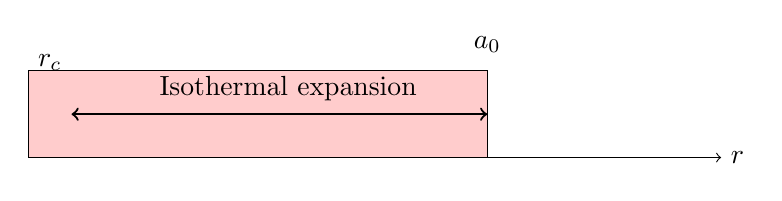
\begin{tikzpicture}[scale=1.1]
                    \draw[->] (0,0) -- (8,0) node[right] {$r$};

                    \draw[fill=blue!30] (0,0.2) rectangle (0.5,0.8);
                    \node at (0.25,1.1) {$r_c$};

                    \draw[fill=red!20] (0,0) rectangle (5.3,1.0);
                    \node at (5.3,1.3) {$a_0$};

                    \draw[<->, thick] (0.5,0.5) -- (5.3,0.5);
                    \node at (3,0.8) {Isothermal expansion};
                \end{tikzpicture}
                \caption{Hydrogen ground-state radius as an isothermal swelling from $r_c$ to $a_0$.}
            \end{figure}

%--------------------------------------------------------------
        \subsection*{F.3 Unruh Echo: Two-Stage Thermodynamic Response}

            \begin{figure}[h!]
                \centering
                \begin{tikzpicture}[scale=1.2]
                    \draw[->] (0,0) -- (7,0) node[right] {$t$};
                    \draw[->] (0,0) -- (0,3) node[above] {Signal};

% primary burst
                    \draw[thick,blue] (0.1,0) -- (0.1,2.5);
                    \node[blue] at (0.1,2.8) {Primary (0.1 ns)};

% echo
                    \draw[thick,red] (3,0) -- (3,2);
                    \node[red] at (3,2.4) {Echo (30 ns)};
                \end{tikzpicture}
                \caption{SST interpretation of Unruh Echo: fast swirl-sector pulse followed by
                slower EM transduction.}
            \end{figure}

%==============================================================
    \section*{References}
%==============================================================

        \begin{thebibliography}{99}

            \bibitem{AbeOkuyama}
            S.~Abe and S.~Okuyama,
            ``Similarity between quantum mechanics and thermodynamics:
            Derivative of the partition function'',
            \emph{Phys. Rev. E} 83, 021121 (2011).

            \bibitem{Kelvin}
            W.~Thomson (Lord Kelvin),
            ``On Vortex Atoms'',
            \emph{Proc. R. Soc. Edinburgh} (1867).

            \bibitem{Helmholtz}
            H.~Helmholtz,
            ``Über Integrale der hydrodynamischen Gleichungen'',
            \emph{J. Reine Angew. Math.} 55 (1858).

            \bibitem{Batchelor}
            G.~K. Batchelor,
            \emph{An Introduction to Fluid Dynamics},
            Cambridge Univ. Press (1967).

            \bibitem{Saffman}
            P.~G. Saffman,
            \emph{Vortex Dynamics},
            Cambridge University Press (1992).

            \bibitem{SSTCanon}
            O.~Iskandarani,
            \emph{Swirl–String Theory: Canon v0.5.12},
            Zenodo (2025).

            \bibitem{HydroHydrogen}
            O.~Iskandarani,
            ``Hydrodynamic Origin of the Hydrogen Ground State'',
            Zenodo (2025).

            \bibitem{DualVacuum}
            O.~Iskandarani,
            ``Hydrodynamic Dual-Vacuum Unification: Swirl Radiation and Photon Torsion'',
            Zenodo (2025).

            \bibitem{UnruhEcho}
            O.~Iskandarani,
            ``Two-Vacuum Interpretation of the Unruh Echo'',
            Zenodo (2025).

        \end{thebibliography}

%==============================================================
% END DEEL III
%==============================================================



\end{document}